\scanpage{35}
\mspage{2}
\textcircled{4} \(\nu=2\). \deleted{Il y a \unsure{deux cas}} \(K^g=\{P\}\), et \(K\setminus K^g\) \inserted{\(=I\)} est réunion de deux orbites. Ainsi, \(g\) est un autom. \deleted{\unsure{de}} ``universel'' de \(\Sigma\setminus I\) (\(g\in V(\unsure{D_I})\)) et \(P\) est \inserted{un de ses} pts fixes. \deleted{\unsure{De}} Cette fois, la situation a des ``modules'', p.ex. en choisissant une des deux orbites,

\deleted{OPS que l’opération de \(g\) sur elle est celle de \(\mu_2\) \inserted{\(=\{\pm1\}\)} sur \(\mu_2\) \inserted{\(=\{\pm1\}\)}, et \(P=0\), l’autre orbite est donnée par un \(\{t,-t\}\), avec \(\lambda=t^2\ne1,\lambda\in k^\times\) ---
donc \deleted{\(\lambda=\)} \(J=(0,\pm1,\pm\sqrt\lambda)\) \deleted{\(\unsure{\sqrt\lambda,\sqrt\lambda}\)}, avec \(\lambda\in\unsure{\mathbb P^1}(k)\setminus\{0,1,\infty\}\),
\unsure{en} \deleted{\unsure{changeant}} changeant le choix de l’orbite, on trouve
\[
(0,\pm1,\pm\sqrt{1/\lambda}).
\]
Prenons le paramètre \(\beta=\lambda+\frac1\lambda\), \inserted{\(\ne2\)}, donc \(\lambda^2-\beta\lambda+1=0\),
\deleted{\(\lambda=\frac12(\beta\pm\sqrt{\beta^2-4})\)},
on trouve \((0,\pm1,\pm\sqrt{\frac12(\beta\pm\sqrt{\beta^2-4})})\).
\unsure{Eliminer} \(0,\infty\), et \unsure{deux} \unsure{discriminant différent} \(2,\infty\) --- \unsure{comme} \deleted{\unsure{les}} \(\lambda\), et
\(g(z)=\frac{\lambda}{z}\), pts fixes.}

Cas moins intéressant que les précédents, de notre point de vue, car il y a des modules. Quand la structure \((\Sigma,I)\) est une structure carrée, on retrouve soit le cas \(2^\circ\) (si \(g\) laisse stables les deux diagonales), soit le cas d’un \inserted{des sommets} \deleted{\unsure{carré}} carré sphérique \unsure{équilatéral}, et du milieu de l’une des arêtes. \inserted{Est-ce le cas \(\unsure{1^\circ|2^\circ}\) ?} Quand c’est une structure tétraédrale, \(P\) est un des \inserted{\(6\)} sommets de l’octaèdre associé.

\figure{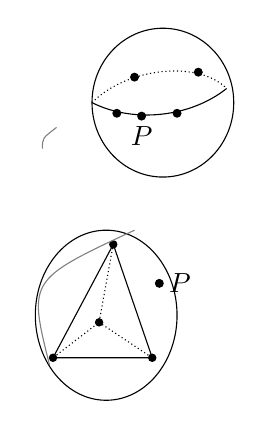
\begin{tikzpicture}[scale=.9]
\draw(0,0)ellipse(1 and 1.05);
\draw(-1,0)..controls(-.4,-.3)and(.4,-.2)..(.9,.2);
\draw[densely dotted](-1,0)..controls(-.5,.5)and(.5,.6)..(.9,.2);
\foreach \x/\y in {-.65/-.15,-.3/-.19,.2/-.15,-.4/.36,.5/.43}{\fill(\x,\y)circle(1.8pt);}
\node[below]at(-.3,-.2){$P$};
\draw[gray](-1.5,-.35)..controls(-1.7,-.5)..(-1.7,-.65);
\begin{scope}[shift={(-.8,-3)}]
\draw(0,0)ellipse(1 and 1.2);
\draw(-.75,-.6)--(.1,1)--(.65,-.6)--cycle;
\draw[densely dotted](.1,1)--(-.1,-.1)--(-.75,-.6);
\draw[densely dotted](-.1,-.1)--(.65,-.6);
\foreach \x/\y in {.1/1,-.75/-.6,.65/-.6,-.1/-.1}{\fill(\x,\y)circle(1.7pt);}
\fill(.75,.45)circle(1.8pt)node[right]{$P$};
\draw[gray](-.8,-.7)..controls(-1.1,.5)..(.4,1.2);
\end{scope}
\end{tikzpicture}}

\uline{Cas des antiautomorphismes de \(\Sigma\)} \inserted{\(\sigma\)} laissant \uline{stables} \(K\). \inserted{(cas \(k=\mathbb C\))} Comme il est d’ordre pair, on voit qu’il \deleted{\unsure{a}} a un pt fixe au moins dans \(K\), \deleted{de} donc \(\Sigma\), et étant d’ordre fini, on voit qu’il est d’ordre \(2\), il correspond à une structure réelle sur \(\Sigma\), \deleted{\unsure{et}}
On distingue suivant le cardinal de \(K^\sigma\), qui est \(1,3\), ou \(5\).
\mspage{34}
